\documentclass[tikz]{standalone}

\usepackage{tikz}
\usepackage{xcolor}
\usepackage{pgfplots}
\usepackage{siunitx}
\usepackage{fontspec}

\pgfplotsset{compat=1.18}

\usetikzlibrary{shapes,arrows,positioning,backgrounds,calc,intersections,calc,svg.path,fit}

\definecolor{ugent-re}{RGB}{220, 78, 40}        % vermilion			/ vermiljoen
\definecolor{ugent-we}{RGB}{45, 140, 168}       % no match
\definecolor{ugent-we-dark}{RGB}{31, 98, 118}       % no match
\definecolor{ugent-ge}{RGB}{232, 94, 113}       % rose				/ bleekrood
\definecolor{ugent-ea}{RGB}{111, 113, 185}      % distant blue		/ verblauw
\definecolor{ugent-pp}{RGB}{251, 126, 58}       % deep orange		/ dieporanje
\definecolor{ugent-ps}{RGB}{113, 168, 96}       % yellow green		/ geelgroen

\begin{document}
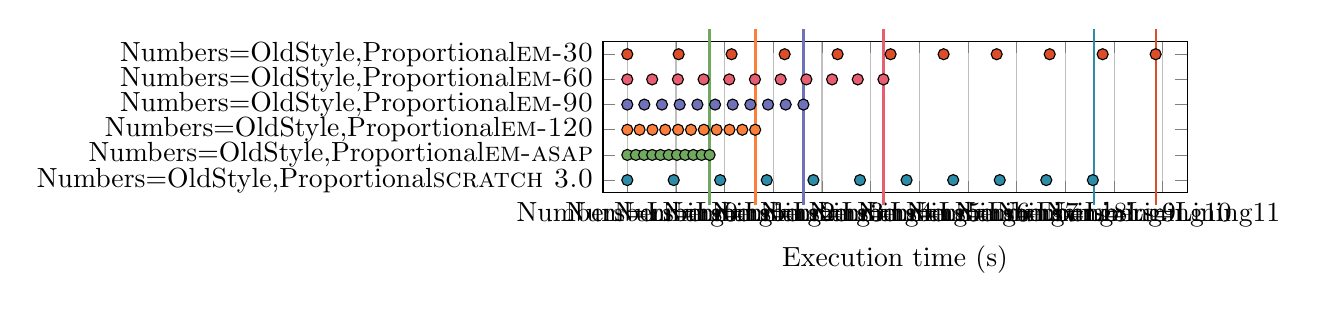
\begin{tikzpicture}
    \pgfplotsset{
        scratch/.style={fill=ugent-we},
        em-30/.style={fill=ugent-re},
        em-60/.style={fill=ugent-ge},
        em-90/.style={fill=ugent-ea},
        em-120/.style={fill=ugent-pp},
        em-asap/.style={fill=ugent-ps},
    }
    \begin{axis}[
        height=3.5cm,
        width=9cm,
        symbolic y coords={min,scratch 3.0,em-asap,em-120,em-90,em-60,em-30,max},
        xtick distance=1000,
        ytick distance=1,
        xmajorgrids,
        xmax=11500,
        xmin=-500,
%        mark size=1pt,
        scaled x ticks=false,
        clip=false,
%        extra x ticks={0},
        xlabel={Execution time (s)},
%        ytick pos=bottom,
%        xtick style={draw=none},
%        axis line style={draw=none},
        yticklabel={\addfontfeature{Numbers={OldStyle,Proportional}}\textsc{\tick}},
        xticklabel={\addfontfeature{Numbers={Lining}}\num[round-mode=places,round-precision=0,fixed-exponent=3,exponent-mode=fixed,drop-exponent=true]{\tick}},
%        xticklabel={\addfontfeature{Numbers={OldStyle,Proportional}}\textsc{\tick}}
    ]
        % em-120
        \addplot[em-120,only marks] coordinates {
            (0,em-120)
            (252,em-120)
            (516,em-120)
            (779,em-120)
            (1044,em-120)
            (1308,em-120)
            (1572,em-120)
            (1835,em-120)
            (2099,em-120)
            (2363,em-120)
            (2627,em-120)
        };
        \draw[color=ugent-pp,line width=1pt] (axis cs:2630,min) -- (axis cs:2630,max);
        \addplot[em-30,only marks] coordinates {
            (0,em-30)
            (1055,em-30)
            (2142,em-30)
            (3232,em-30)
            (4320,em-30)
            (5409,em-30)
            (6498,em-30)
            (7588,em-30)
            (8677,em-30)
            (9765,em-30)
            (10854,em-30)
        };
        \draw[color=ugent-re,line width=1pt] (axis cs:10861,min) -- (axis cs:10861,max);
        \addplot[em-60,only marks] coordinates {
            (0,em-60)
            (511,em-60)
            (1039,em-60)
            (1567,em-60)
            (2094,em-60)
            (2622,em-60)
            (3150,em-60)
            (3679,em-60)
            (4207,em-60)
            (4734,em-60)
            (5262,em-60)
        };
        \draw[color=ugent-ge,line width=1pt] (axis cs:5268,min) -- (axis cs:5268,max);
        \addplot[em-90,only marks] coordinates {
            (0,em-90)
            (350,em-90)
            (712,em-90)
            (1076,em-90)
            (1440,em-90)
            (1803,em-90)
            (2165,em-90)
            (2528,em-90)
            (2891,em-90)
            (3254,em-90)
            (3618,em-90)
        };
        \draw[color=ugent-ea,line width=1pt] (axis cs:3624,min) -- (axis cs:3624,max);
        \addplot[scratch,only marks] coordinates {
            (0,scratch 3.0)
            (953,scratch 3.0)
            (1908,scratch 3.0)
            (2865,scratch 3.0)
            (3823,scratch 3.0)
            (4780,scratch 3.0)
            (5737,scratch 3.0)
            (6695,scratch 3.0)
            (7651,scratch 3.0)
            (8607,scratch 3.0)
            (9564,scratch 3.0)
        };
        \draw[color=ugent-we,line width=1pt] (axis cs:9586,min) -- (axis cs:9586,max);
        \addplot[em-asap,only marks] coordinates {
            (0,em-asap)
            (176,em-asap)
            (344,em-asap)
            (512,em-asap)
            (682,em-asap)
            (852,em-asap)
            (1020,em-asap)
            (1188,em-asap)
            (1356,em-asap)
            (1526,em-asap)
            (1691,em-asap)
        };
    \draw[color=ugent-ps,line width=1pt] (axis cs:1694,min) -- (axis cs:1694,max);
    \end{axis}
\end{tikzpicture}
\end{document}
